\part{Analysing within- and between-host phylogenies}

The tree analysis procedure takes as input one or more phylogenies, and analyses them to reconstruct transmission, and identify multiply infected individuals and contaminants.
In order, the following steps are performed:

\begin{enumerate}
\item  Identify and exclude tree tips corresponding to reads that should not be used to reconstruct transmission (blacklisting)
\item Perform an ancestral state reconstruction on each tree in turn, and use this to identify host subgraphs (contiguous regions of the phylogeny that have been assigned to the same host)
\item Calculate per-host summary statistics, and graph them across the genome if multiple trees are given as input
\item In each tree, determine the relationship between each pair of hosts determined by the relative positions of their subgraphs
\item Summarise these pairwise relationships over all trees (if more than one tree was given).
\end{enumerate}

The code forms an \c{R} package entitled \c{phyloscannerR} which appears as a subfolder in the \p directory. The package manual can also be found in this directory and users who prefer to perform the analysis within \c{R} itself may wish to consult that. This package and its dependencies must be installed prior to use, whether within \c{R} or at the UNIX command line; all dependencies are available in \href{http://cran.r-project.org/}{CRAN} except for \c{ggtree}~\cite{MEE3:MEE312628}, which is part of \href{http://bioconductor.org/}{Bioconductor}.

To install \c{phyloscannerR} (and \c{ggtree}), use the command line to navigate to the ``phyloscannerR'' subdirectory of the ``phyloscanner'' directory, then start \c{R} and enter the following commands:
\begin{verbatim}
> install.packages("devtools")
> library(devtools)
> source("https://bioconductor.org/biocLite.R")
> biocLite("ggtree")
> install("../phyloscannerR", dependencies = T)
\end{verbatim}
(Obviously if you have already installed \c{ggtree} then the second and third lines can be skipped.) 


A single command line script, \pat, can be used to perform a full analysis.
Each step identified above also has its own standalone script, which can be used to, for example, analyse multiple trees in parallel on a cluster.
We do not document all the command line options for these additional scripts here, and the user is directed to their \c{--help} options.

\section{The basic command}

The basic command for \pat is
\begin{verbatim}
$ phyloscanner_analyse_trees.R TreeInput OutputString ReconstructionModeArguments
\end{verbatim}
\c{OutputString} is simply a string identifying all file output.
The tree input can be either a single tree file or a single string that begins all files (see below).
For full instructions regarding\break \c{ReconstructionModeArguments}, see section~\ref{sec:ParsimonyReconstruction}; for a quick start, \c{s,0} gives a parsimony reconstruction with no within-host diversity penalty.
However, be aware that this version of the algorithm will not be aware of potential contamination.

\section{Name format for input files}

Tree files should be in Newick or Nexus format.
These can be the product of\break \pmt, but need not be; the script will work on any set of trees if the tip labels can be interpreted properly (see below).
Each tree should reside in a single file.

The tree files, when the analysis is to be performed on multiple trees, are expected to all be located in the same directory and have names that all begin with the same nonempty string.
The remainders of the file names, excluding the file extensions, are referred to as file suffixes.
If the genome window approach is used (i.e. each tree represents a window of the genome), the suffixes will be expected to contain the coordinates of the genome window for each tree.
(Output from \pmt will automatically be formatted in this way.) A regular expression described below (see section~\ref{sec:regexes}) is used to identify these coordinates; if it fails to identify them, then the script will assume that the windowed approach was not used.

Any accompanying per-window files specified in optional arguments are assumed to follow the same pattern: a string beginning every file, the same set of suffixes, and a file extension.
This will automatically be the case for files produced by \pmt: the values of the recombination metric (see section~\ref{sec:SumStats}), and the list of reads that are identical amongst different hosts (see section~\ref{sec:DupBlacklisting}).
Any user-specified blacklists (see section~\ref{sec:UserBlacklisting}) must also have file names in this format.

Tree files are by default assumed to have \c{.tree} as a file extension and csv files \c{.csv}, but this can be overridden with the \c{--treeFileExtension} and \c{-csvFileExtension} options.

If the analysis is instead to be performed on a single tree, the file name of that tree should be given as the \c{TreeInput} argument instead.
The same goes for any other files to be used as optional arguments.

\section{Output}

The default output of \pat varies depending on whether it is run on one or multiple trees.

If the input is a single tree file, the default output is an annotated pdf version of that tree, a csv file of summary statistics for the hosts present in that tree, and a csv file outlining the relationship between each pair of hosts in that tree.

If the input is multiple trees, then the default output is an annotated pdf version of all trees, a csv file of summary statistics for every host across all the trees, a pdf graphing those statistics across all trees, and a csv file summarising which pairs of hosts meet the criteria for being closely related.

\section{Preparing the trees}

Two options determine processing of the phylogeny before any further operations are performed.
A named outgroup can be specified with \c{--outgroupName}; this is recommended unless the input trees are known to be correctly rooted.
It is always assumed that the lineage represented by the root of the entire phylogeny was not present in any sampled host, even if no outgroup is given.
Trees output by \pmt will need to be re-rooted

The output of many phylogeny reconstruction packages, including \R, is a binary phylogeny.
While multifurcations may seem to appear when the trees are viewed by eye, these will have a hidden binary branching order.
The branches connecting the nodes within these ``multifurcations'' may all be of an extremely short but nonzero minimum length (in \R output) or actually zero length (in, e.g., PhyML output).
Since this branching order is largely arbitrary, it is recommended that these regions of the tree be collapsed into genuine multifurcating nodes for \pat.
A length threshold to determine pairs of nodes that should be so collapsed can be specified with \c{--multifurcationThreshold}.
This is normally numerical, but if \c{g} is given it will be guessed from the trees itself. If the trees have interpretable genome window coordinates, the smallest branch length will be compared to the branch length corresponding to one SNP. If the former is smaller than 0.25 times the latter, the former will be used as the threshold; if not, the tree is assumed to contain no multifurcations and no collapsing is done. If no genome window coordinates are available, the shortest branch length is simply used as the threshold. Before specifying \c{g} the user should ideally ensure that the trees genuinely do contain apparent multifurcations.

\section{Tip label and file suffix regular expressions} \label{sec:regexes}

The tip labels in the input phylogenies are expected to follow a regular expression that identifies host IDs, and optionally also read identifiers and read counts.
The exact format is specified using a regular expression with three capture groups: for host ID, read ID, and count.
The count is expected to be an integer.
If a third group is not found then it assumed that every tip represents only a single read.
The default regular expression is \verb|"^(.*)_read_([0-9]+)_count_([0-9]+)$"|, but the user can specify an alternative with the \c{--tipRegex} option.
In plainer language, this is of the form ``NAME\_read\_X\_count\_Y'' where NAME is the host name, X the read identifier and Y the read count.
The tip names of the outgroup (if it exists), and of any other reference sequences that are included, should not match this regular expression.

The default regex is appropriate for analysing trees output by \pmt, when each bam contains reads from a different host.
A different regular expression may be required if the input is not from \pmt.
It may also be required for trees output by \pmt if multiple bam files contain sequences derived from the same host, and part of the bam file name identifies the host.
For example if you had three bam files named \mbox{PatientA-1.bam}, PatientA-2.bam and PatientB-1.bam, where tips from the first two are from the same host.
Changing the tip regex to \verb|"^(.*)-[0-9+]\\.bam_read_([0-9]+)_count_([0-9]+)$"| means that the first group in the regex will match ``PatientA'', ``PatientA'' and ``PatientB'' for the three bams respectively; all tips from the first two bams are then associated to the same host, PatientA.

Similarly, the set of file suffixes (see above) may contain genome window coordinates, and a regular expression is used to identify these.
Two capture groups are expected for the start and end of the window.
The default is \verb|"^\\D*([0-9]+)_to_([0-9]+)\\D*$"|.
In plainer language this is any number of non-digit characters, followed by ``X\_to\_Y'' where X is the window start and Y the end, followed by any number of non-digit characters.
An alternative can be specified with the \c{--fileNameRegex} option.

\section{Branch length normalisation} \label{sec:normalisation}

Two hosts may be classified as closely linked by \pat on the grounds that they have host subtrees separated by a patristic distance that lies below a given threshold.
However because we are often interested in a genomic window approach, a fixed distance threshold for all trees may not be appropriate because of variations in nucleotide diversity in different areas of the genome.
This is because a distance threshold suggestive of a close epidemiological relationship in one window will not be in others.
To remedy this, \pat can be asked to normalise branch lengths across windows.

One approach to generating appropriate normalisation values over the genome is implemented by the script \c{tools/CalculateTreeSizeInGenomeWindows.py}.
Run from the command line (see it's \c{--help} option for details on how) taking a whole-genome alignment of existing reference sequences as input, it infers phylogenies in sliding windows, and characterises the size of the tree by taking the median of the set of patristic distances between all pairs of references.
One such value is obtained per window; one value is then assigned to each integer position in the genome by taking the mean of the values from those windows spanning this position (with windows chosen to overlap, so that multiple values for each position should smooth some stochasticity in phylogenetic inference).

Q: what alignment of existing reference sequences should you use for this?
A: ideally, one which is in some sense representative of between-host diversity.
We find all pairwise patristic distances, so if your set of sequences is biased to be overly representative of a particular subset, these patristic distances will become biased towards zero.
That said, all we're interested in here is how patristic distances change across the genome, not their absolute values.

The output from \c{tools/CalculateTreeSizeInGenomeWindows.py}, or alternatively any other csv file containing genomic positions with associated normalisation constants, can be used with the\break \c{--normRefFileName} option.
This will scale all normalisation constants by the same factor such that their mean is 1.
A normalisation constant is then determined for each window by taking the mean of the values for all positions in the window.
This constant for the window is used to scale all branch lengths in the tree for subsequent processing by \pat.
The similar option \c{--normStandardiseGagPol}, specific to HIV genomes, instead scales normalisation constants so that the mean of the constants on the {\it gag} and {\it pol} genes is 1; distances anywhere in the genome are then interpretable as standard distances in {\it gag/pol}.
Both of these options assume that window coordinates are present in file suffixes.
Note that the genomic coordinates specified here must mean the same thing as the window coordinates in the file suffixes.
As discussed in section~\ref{sec:CoordMeaning}, window coordinates in tree file names output by \pmt may mean one of two things -- they may be with respect to a named sequence or with respect to an alignment.

The \c{--normalisationConstants} option is used to directly specify the normalisation to be used for each tree file.
If the argument is numerical, it is used as a normalising constant for every tree.
If it is instead the path to a .csv file, then this file is expected to consist of a first column listing all input tree file names, and a second of normalising constants.
The presence of \c{--normalisationConstants} overrides any other normalisation options, which will be disregarded.

The standalone script \c{normalisation\_lookup\_writer.R} can be used to separately write a .csv file for use with the \c{--normalisationConstants} option using the procedure described in this section. This is not normally necessary for use of \pat, but can be used as an argument for other standalone scripts.

The normalisation is used for the parsimony reconstruction (see section~\ref{sec:ParsimonyReconstruction}) and for the identification of closely-related hosts (see sections~\ref{sec:Classification} and \ref{sec:ClassificationSummary}). However, output trees have the same branch lengths as input trees, and summary statistics (see section~\ref{sec:SumStats}) are calculated using raw branch lengths.

\subsection{Parallelising \texttt{tools/CalculateTreeSizeInGenomeWindows.py}}
The \c{--threads} option of \c{tools/CalculateTreeSizeInGenomeWindows.py} can be used to specify multiple threads, allows multiple windows to be analysed in parallel using multiple cores on the same machine.
Alternatively, power users may want to massively parallelise, e.g. over multiple different machines on a computing cluster.
Read on if interested; skip ahead to section~\ref{sec:Blacklisting} if not.
First choose your desired start, end, window width and increment parameters.
Then generate a set of \\\c{tools/CalculateTreeSizeInGenomeWindows.py} commands, with each command running only a single window, namely the window after the one of the previous command.
For example say you wanted to start at position $1000$, end at $9000$, have a window width of $300$ and an increment of $10$.
Your first window is $1000-1299$, your second is $1010-1309$, $\ldots$ and these can be run as separate commands thus:
\begin{verbatim}
$ tools/CalculateTreeSizeInGenomeWindows.py MyAln.fasta MyChosenSeqName \
  1000 300 output_1000-1299 -E 1299
$ tools/CalculateTreeSizeInGenomeWindows.py MyAln.fasta MyChosenSeqName \
  1010 300 output_1010-1309 -E 1309
...
\end{verbatim}
Generating these commands is easily done as part of a loop, e.g.
\begin{verbatim}
$ for start in $(seq 1000 10 8700); do
$   end=$((start + 299))
$   command="tools/CalculateTreeSizeInGenomeWindows.py MyAln.fasta MyChosenSeqName"\
" $start 300 output_${start}-${end} -E $end"
$ done
\end{verbatim}
and each command could be put inside a separate file to be run as a separate job.
In this example, output files will be produced named \c{output\_1000-1299\_ByWindow.csv}, \c{output\_1000-1299\_ByWindow.csv}, $\ldots$; these can be combined with
\begin{verbatim}
$ cat output_*_ByWindow.csv | sort -n | uniq > output_all_ByWindow.csv 
\end{verbatim}
(the \c{sort} and \c{uniq} commands preventing the csv header repeating).
Finally, running
\begin{verbatim}
$ tools/FromPerWindowStatsToPerPositionStats.py output_all_ByWindow.csv \
  > output_all_ByPosition.csv
\end{verbatim}
converts the per-window tree sizes to per-position tree sizes, as required as input for the\break \c{--normRefFileName} option of \pat.

(We used this approach for parallelisation, as we covered the HIV genome with windows of width 301 bp and an increment of 1 bp, necessitating 9179 windows.
Running these as 9179 separate commands in parallel on a cluster sped things up considerably.)

\section{Blacklisting} \label{sec:Blacklisting}

Blacklisting refers to the exclusion of some tips in the phylogeny from the full analysis.
This may be done for a variety of reasons:
\begin{itemize}
\item Tips from suspected contaminant reads (i.e. for which we suspect the true host is not the recorded host) should not be used to reconstruct transmission
\item Possible multiple infections may complicate an analysis and the user may prefer to deal only with the largest collection of reads from such a host
\item Uneven tip or read counts between different hosts have the potential to bias the inference of transmission.
The user may wish to remove some tips in order to mitigate this.
\end{itemize}
\p includes a number of utilities to perform blacklisting, all of which can be run as part of \pat.
The script does all blacklisting internally, but other scripts in the \c{tools} directory of the \p code can be used to generate lists of suspect tips in an input phylogeny. In addition, a script entitled \pcl may be used to perform blacklisting and remove blacklisted sequences from the input alignments without performing a full \p run; see the \c{--help} for this for more details.
The various types of blacklisting are listed below.
All, except user blacklisting, assume that the tree tips are annotated with read counts.

A CSV file listing every tip that was blacklisted in every tree, and why, will be output if the \c{--blacklistReport} option is given to \pat.

\subsection{Duplicate blacklisting} \label{sec:DupBlacklisting}

This procedure blacklists reads from one host which are identical to reads from another, but are present in sufficiently small numbers that it would be suspected that they are merely contaminants.
It is enabled with the \c{--duplicateBlacklist} option to \pat, which takes a single argument identifying the duplicate output files from \pmt.
Tips are blacklisted if the corresponding sequence is exactly identical to the sequence for a tip from another host, and either the raw read count from the former tip, or the ratio of the read count from the former tip to the read count from the latter tip, is less than a specified threshold.
The raw read count is specified with the \c{-rwt} option and the ratio threshold with the \c{-rtt} option.
It is acceptable to specify both.
As the default values for both are 0, nothing will be blacklisted unless at least one is given a positive value.

\pat will append ``\_X\_DUPLICATE'' to the tip names of tips blacklisted by this procedure, which will appear in annotated tree output.
The standalone R script is \c{duplicate\_blacklister.R}.

\subsection{Parsimony-based blacklisting for contaminants}

While in many cases contaminant reads will be identical to those from another host in the dataset, the user may not always be so fortunate; the contaminant may be from another dataset entirely, and hence have no exact matches amongst the reads that are used to reconstruct the phylogeny.
Similarly, a variant may be sequenced from the dataset that is never assigned the correct host.
The \c{--parsimonyBlacklistK} option to \pat can be used to identify such tips, using the same parsimony procedure that is employed for ancestral state reconstruction (see section~\ref{sec:ParsimonyReconstruction}, and the \p paper).
The single additional numerical argument to \c{--parsimonyBlacklistK} is the value of $k$ used to calculate a within-host diversity penalty.

We use this procedure because excessive amounts of within-host diversity may be just as suggestive of contamination as of a genuine multiple infection.
For each host in turn, the tree is pruned so that only the tips from that host, and the outgroup, remain.
(If no such outgroup is given,\break \pat will attempt to find one.) The reconstruction is them performed on this pruned tree, using the $k$ parameter specified with \c{--parsimonyBlacklistK}, and the result used to see whether the tips of the tree were grouped into one subgraph or more than one subgraph.
If the former, then the phylogeny does not suggest sufficient diversity within this host to suggest either a multiple infection or contamination.
If the latter, then one or the other is likely to be true.
We suggest that a subgraph is more likely to be contamination when it contains very few reads.
The arguments used in duplicate blacklisting are reused here.
If the total number of reads associated with the tips in a subgraph is smaller than the raw threshold (\c{--rawBlacklistThreshold}), then all tips in the subgraph are blacklisted.
If the proportion of reads from the host that belong to a subgraph is smaller than the ratio threshold (\c{--ratioBlacklistThreshold}), then all tips in that subgraph are blacklisted.
The former threshold is applied even if there is only one subgraph, in which case it is assumed that so few reads exist from the host in question that all of them could well be contaminants, with genuine sequencing failing in this part of the genome.

\pat will append ``\_X\_CONTAMINANT'' to the tip names of tips blacklisted by this procedure, which will appear in annotated tree output.
The standalone R script is \c{parsimony\_based\_blacklister.R}.

\subsection{Dual infection blacklisting}

If the parsimony-based blacklisting procedure identifies a host with suspicious amounts of within-host diversity where the smaller subgraphs have too many reads to be flagged as likely contaminants, a dual infection (or larger multiple infection) may be suspected.
The current version of\break \pat is only able to summarise the relationships of such a host with the neighbours of all its subgraphs in the transmission tree; it cannot separate the neighbours of each subgraph.
This may result in spurious inferences being drawn, where a close neighbour to one subgraph and a close neighbour to another are identified as closely related to each other.
If this behaviour is regarded as particularly undesirable, a suggested stopgap remedy is to assume that the subgraph with the largest read count represents the same infection across the entire genome, and blacklist the rest.

The \c{--dualBlacklist} flag, which can be used only if \c{--parsimonyBlacklistK} is also specified, will do this blacklisting.
\pat will append ``\_X\_DUAL'' to the tip names of tips blacklisted by this procedure, which will appear in annotated tree output.
 The standalone R script is \c{dual\_host\_blacklister.R}.

\subsection{User blacklisting} \label{sec:UserBlacklisting}

The user may wish to specify his or her own blacklist before \pat is run.
A separate plain text file for each window should be prepared, with a blacklisted tip on each line, ending with the same file suffix as the corresponding tree file. The path to these files and the string beginning each should be specified with the \c{--userBlacklist} option.
These tips will be blacklisted from the start, and \pat will append ``\_X\_USER'' to tip labels.

\subsection{Downsampling}

The intention of the downsampling procedure is to ensure that the same numbers of reads are included in the analysis from each host in the dataset.
This is done by taking a random sample of reads, without replacement, and blacklisting tips where the corresponding reads was never selected at all.
 The \c{--maxReadsPerHost} option is used to specify a number of reads to downsample to.
If \c{--blacklistUnderrepresented} is specified then hosts without enough reads in totality are blacklisted, but if it is absent then all tips from those hosts are retained.

\pat rewrites tip labels to reflect the number of times a tip was randomly selected.
``\_X\_DOWNSAMPLED'' is appended to tips that are blacklisted because the corresponding reads were never selected, in which case the read count in the tip label will have been rewritten to 0.
``\_X\_UNDERREPRESENTED'' is appended to those that are blacklisted because they are from a host without enough reads in total (if \c{-dsb} is given).
The standalone R script is \c{downsample\_reads.R}.

\subsection{Pruning the blacklist}

Default behaviour is to leave blacklisted tips in the phylogeny; they are not annotated with any host and are instead given the unsampled state in the parsimony reconstruction, but they remain so as to be examined in the annotated tree output.
The \c{--pruneBlacklist} option to \pat can be used to prune these tips instead, in which case they will not appear in output at all.

\section{Parsimony reconstruction} \label{sec:ParsimonyReconstruction}

The core of the \pat analysis is an ancestral state reconstruction of hosts to internal nodes of each phylogeny.
We offer several algorithms for this; the exact one is specified with the final compulsory argument to \pat.
For full details, see the supplementary information of the \p paper.
\begin{itemize}
\item A fast, non-rigorous (for more than two hosts) adaptation of the procedure outlined in Romero-Severson et al. (PNAS 2016).
This is specified by \c{r}.
It will not reliably reconstruct multiple infections.
\item A parsimony reconstruction using the Sankoff algorithm that allows for an additional ``unassigned'' state and can be configured to penalise the reconstruction of single infections to hosts which imply unreasonable amounts of diversity.
This is specified by two or three arguments, separated by commas.
The first is \c{s}.
The second is the value of the $k$ parameter that penalises within-host diversity; if this is set to 0 then no penalty is applied and the procedure is equivalent to standard parsimony with the unassigned state.
It is recommended that users explore their data to pick suitable values of $k$, as it is likely to be pathogen- and sequencing method-dependent. As a rule of thumb, it should be the reciprocal of a patristic distance so large that it would be surprising to encounter a host with an infection so diverse that a phylogeny built from pathogen sequences from just that host had a branch that long or longer, if the host was infected only once.
\end{itemize}
The latter parsimony reconstruction algorithm uses a very large matrix for large trees and occasionally \c{R} will run out of memory; the argument \c{--useff} will cause the script to use the \c{ff} library instead, which solves many memory issues at the cost of speed.

Of concern in either of the two proper parsimony reconstruction algorithms is used is how to handle terminal branches of zero or negligible length.
In particular, if a tip with a read count of $n$ is connected to its parent node by such a branch, should that tip be considered as one tip or $n$ tips for the parsimony reconstruction? As an illustrated example, see below.
Phylogenetic software output, with minimum-length branches collapsed to zero (see above) might appear as in diagram a) in Fig.~\ref{fig:ZeroLengthBranches} below, where colours represent hosts and the numbers in the coloured tips read counts, while numbers on branches are branch lengths (with zero-length branches displayed with nonzero lengths for clarity).
The question is whether a parsimony reconstruction should consider this clade as b), where all the reads represented by the blue tip in a) form separate tips but their MRCA $m$ is not the MRCA $n$ of the entire clade, or b), where the MRCAs are the same.
Under simple parsimony, the cost of reconstructing $n$ as red is 1 in b) and 3 in c), but the cost of reconstructing it as blue is 2 in both.
By default, \pat treats this situation as b), which is the same as ignoring read counts in the parsimony reconstruction - as it will always be most parsimonious to reconstruct $m$ as blue to avoid turning one transition into three, the three blue tips can be ignored and the colour of $m$ fixed, so we are back to diagram a) - but the \c{--readCountsMatterOnZeroLengthBranches} option, if specified, will treat it as c) instead.

\begin{figure}[!h]
\centering
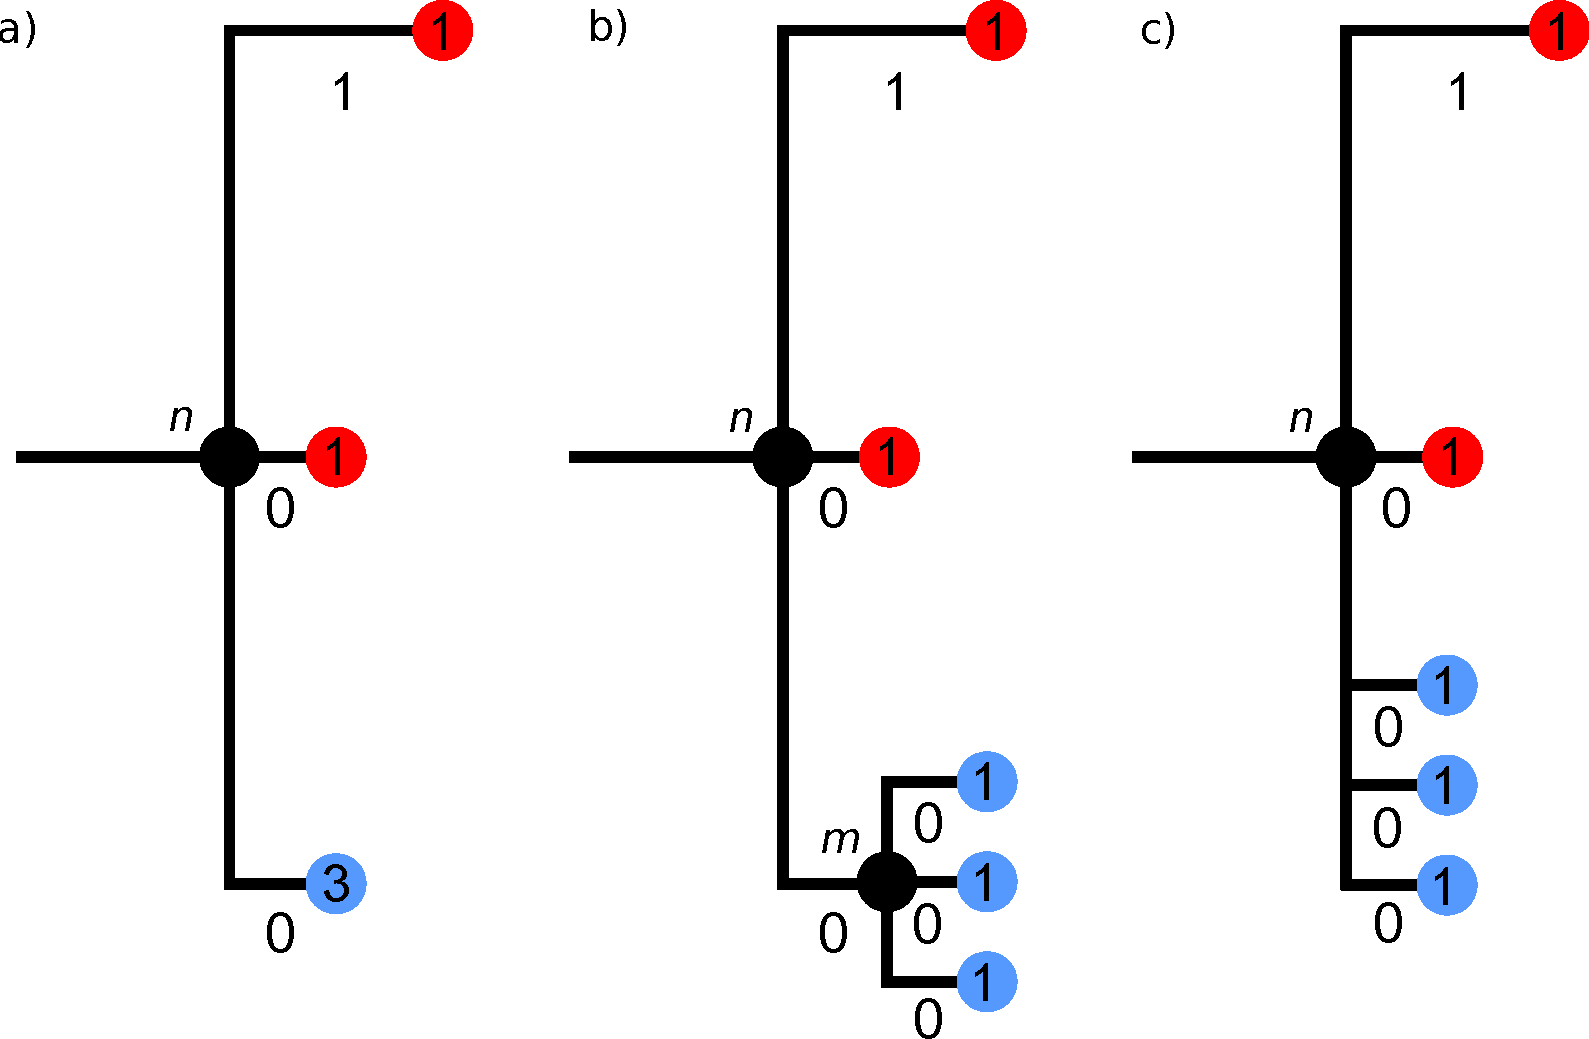
\includegraphics[width=0.6\textwidth]{manualfigure.pdf}
\label{fig:ZeroLengthBranches}
\end{figure}

Annotated versions of all input trees will be output by \pat, in pdf format by default.
The \c{--outputNexusTree} option can be used to make it provide these trees in Nexus format instead.

The standalone R script to perform parsimony reconstruction is \c{split\_hosts\_to\_subtrees.R}.

\section{Summary statistics} \label{sec:SumStats}

By default, \pat produces a csv file of summary statistics with the following columns:
\begin{itemize}
\item id: the host ID for the statistics in this row.
\item file\_suffix: the file suffix of the associated tree file.
\item xcoord: used to draw the graphs (see below); this is the midpoint of the genome window if the windowed approach is used, and the position of the file\_suffix in an alphabetical ordering if not.
\item Tips: the number of tips from this host in this tree.
\item Reads: the number of reads from this host in this tree (if read counts were not detected then this column will be identical to the tip counts, as each tip is assumed to represent one read).
\item Subgraphs: the number of subgraphs that the parsimony reconstruction identified for this host in this tree.
\item clades: the number of separate clades monophyletic clades from this host in this tree.
\item overall.rtt: the mean patristic distance from tips from this host to the MRCA of the tips from this host, weighted by read counts if these are given
\item largest.rtt: the mean patristic distance from tips from the largest (by read count) subgraph from the host to the MRCA of that subgraph, weighted by read counts if these are given.
\item max.branch.length: the length of the longest branch in the tree obtained by pruning all tips from the tree except the ones from this host.
\item max.patristic.distance: the largest patristic distance between any pair of tips from this host.
\item global.mean.pat.distance: the mean patristic distance between tips from this host.
\item subgraph.mean.pat.distance: the mean patristic distance between tips in the largest subgraph.
\item recombination.metric: this column only appears if the recombination metric files output by \\\pmt have been given to \pat using the \\\c{--recombinationFiles} argument.
It gives the value of the recombination metric for this host in this tree.
\item prop.gp.1 to prop.gp.X: A variable number of columns recording what proportion of the reads from this host occur in each subgraph, ordered by size.
The total number of columns is the largest number of subgraphs present for any host in any tree (and so many columns will be 0 for most hosts).
\end{itemize}

Also generated, if more than one phylogeny is given as input, is a pdf file graphing these statistics across all trees for every host.
Each host occupies a separate page in this file, with five or six graphs per host:
\begin{enumerate}
\item Number of reads and number of tips
\item Number of subgraphs and number of clades
\item Mean root-to-tip distance in the largest subgraph and in the whole tree
\item Mean pairwise patristic distance in the largest subgraph and in the whole tree
\item The proportion of reads appearing in each subgraph
\item (If recombination metric files are specified with \c{-R}) The value of the recombination metric across the genome
\end{enumerate}

If the script could detect genome window coordinates from the file suffixes, and the starts and ends of those windows occur regularly across the genome, these graphs will be annotated with light grey rectangles for windows where a host is missing from a single window, and dark grey rectangles where a window appears to be entirely missing (i.e. it had no tree file).

The standalone R script to produce summary statistics is \c{summary\_statistics.R}.

\section{Classification of pairwise relationships}\label{sec:Classification}

The parsimony reconstruction has annotated all internal nodes in each phylogeny with either a host or the unassigned state, and from this information, host subgraphs have been identified.
The next step in the script is to document the relationships between each pair of hosts in every tree.
By default (when the script is run on multiple tree files) this is done silently, but two types of output file can be generated.

The \c{--collapsedTrees} option produces the collapsed tree (see the \p paper), in csv format.
This file has four columns:
\begin{itemize}
\item The collapsed tree node ID, which is the host ID or ``unassigned\_region'' followed by \c{-S} and an identifying number
\item The collapsed tree node ID of that node's unique host, or ``root'' if it has none
\item The ID for the host, or ``unassigned\_region'', associated with this node
\item The ID for the host, or ``unassigned\_region'', associated with the parent node
\end{itemize}

If the script is run on a single tree file only, the classification csv file is produced by default, but the collapsed tree is not.

The \c{--allClassifications} option produces per-tree csv files describing all pairwise relationships between hosts.
The columns of this file are as follows:
\begin{itemize}
\item host.1, host.2: the pair of hosts.
The order does not signify anything on its own but is relevant to interpretation of the path.classification column.
\item adjacent: This is TRUE if there exist two nodes, one each from subgraphs from the two hosts, such that the path between the two traverses only nodes that are either also from these host subgraphs, or unassigned.
(In other words, it is possible to move through the phylogeny from one host to the other without moving through the subgraph of another sampled patient.)
\item contiguous: This is TRUE if for any two nodes, one each from subgraphs from the two hosts, the path between the two intersects no nodes that are not either also from these host subgraphs, or unassigned.
This is similar to adjacent but a little stronger.
\item paths12, paths21: paths12 is the number of nodes from host.2 in the collapsed tree which have an ancestor that is from host.1, and paths21 is the opposite.
\item nodes1, nodes2: these are the number of collapsed tree nodes for host.1 and host.2 respectively.
\item path.classification: this describes the topological relationship between the two hosts in the cablollapsed tree: \begin{itemize}                                                                                                                    
\item ``none'' indicates that no nodes from host.1 are ancestral to nodes from host.2 or vice versa
\item ``anc'' indicates that there is only one node from host.2 and it is a descendant of a node from host.1
\item ``desc'' indicates that there is only one node from host.1 and it is a descendant of a node from host.2
\item ``multiAnc'' indicates that there is more than one node from host.2 and all are descended from a node from host.1
\item ``multiDesc'' indicates that there is more than one node from host.1 and all are descended from a node from host.2
\item ``complex'' indicates that none of the above are true (which is suggestive of an ancestral relationship and often direct transmission, but with unknown direction)
\end{itemize}
\item min.distance.between.subgraphs: this is the smallest  patristic distance between a node in a host.1 subgraph and a host.2 subgraph
\item normalised.min.distance.between.subgraphs: If the tree branch lengths were normalised, this is the above distance but divided by the normalisation constant for this tree
\end{itemize}

The standalone script to classify pairwise host relationships is \c{classify\_relationships.R}.

\section{Pairwise relationship summary}\label{sec:ClassificationSummary}

The next stage in the script is to gather the pairwise relationships between hosts in each window and summarise this across the whole run.
Pairs are inferred to be related in a tree if they are both adjacent and (optionally) within the patristic distance threshold specified by the \c{--distanceThreshold} option.
If \c{--distanceThreshold} is not given then it is assumed to be infinite and adjacency is the only criterion that will be used to identify related pairs.
If tree branch lengths were normalised then the distance threshold is applied to normalised distances.

By default, two outputs are produced. The first is a \c{.csv} file whose first three columns are a pair of hosts and a classification of the topological relationship between the pair.
Rows for pairs which are never related at all or never show a particular topological relationship are omitted.

The \c{--windowThreshold} option is used to specify the minimum proportion of trees in which a pair of hosts were found to be related to make rows for that pair appear in the output file. The default is 0.5, meaning that only pairs that are related in at least half of the trees appear. If this is instead set to 0, all relationships are reported if they ever occur at all.

The \c{.csv} file has the following columns:
\begin{itemize}
\item host.1, host.2: the two hosts.
\item ancestry: the type of ancestry (see below).
\item ancestry.tree.count: the number of trees in which this pair of hosts are related (by the definition given above) and the relationship is of the type given under ``ancestry''.
\item both.exist: the number of trees in which both hosts are present.
\item fraction: the number of windows showing this relationship over the number of windows where both occur (``count'' over ``both.exist''), as text.
\item any.relationship.tree.count: the number of trees in which this pair of hosts are related (by the definition given above).
\end{itemize}

The ancestry relationships are as follows:
\begin{itemize}
\item ``none'': no node in the collapsed tree from host.1 is descended from a node from host.2 or vice versa.
\item ``trans'': there is just one collapsed tree node from host.2 and it is descended from a node from host.1.
Since they must be adjacent, this makes host.1 its immediate ancestor.
\item ``multi\_trans'': there is more than one collapsed tree node from host.2 and all are descended from a node from host.1.
This classification only appears if the \c{--allowMultiTrans} option is given; if not these relationships count as ``complex''.
This is because this relationship is less indicative of the direction of transmission than ``trans''; it may simply indicate that the tips from the two hosts are very intermingled, and it is prone to bias introduced by differences in tip counts.
By default, the script is conservative and does not take this relationship as a signal of directionality.
However, as with ``complex'', it is quite strongly indicative of direct transmission (Romero-Severson et al. PNAS 2016).
\item ``complex'': where none of the above are true; if \c{--allowMultiTrans} is not specified then\break ``multi\_trans'' relationships are also allocated ``complex''.
\end{itemize}
The standalone script to summarise these relationships is \c{transmission\_summary.R}.

Unless the \c{--skipSummaryGraph} option is specified, a PDF file displaying a simplified summary of between-patient relationships will also be produced. The dimensions of this plot (in inches) can be controlled with the \c{--summaryPlotDimensions} options; the default here is $25\times25$ inches. If the output plot is too small and cluttered, try using a larger number. The output here will simplify the between-host relationships as in figure 4B of the \p paper, such that there is only one link between any pair, and that link will appear as an arrow if the proportion of windows showing transmission in that direction is above a threshold, but simply as a line otherwise. Links with arrows are labelled with two numbers separated by a forward slash: the first is the proportion of trees showing the directional relationship implied by the arrow, while the second is the proportion of trees showing any relationship at all. Links without arrows are just labelled with a the proportion showing any relationship. The default threshold for the display of arrows is 0.33, but this can be overridden with the \c{--directionThreshold} option. Links will only appear at all if a relationship occurs in more that the \c{--windowThreshold} option, and it is required that \c{--directionThreshold} be less than or equal to \c{--windowThreshold}.

Graph visualisation is a complicated affair, and we cannot ensure that this PDF file will always display a satisfactory arrangement of nodes and labels. Users wishing to make their own graphs may use an analysis package such as \href{http://www.cytoscape.org/}{Cytoscape} with the summary \c{.csv} file as input. A standalone script, \c{simplify\_graph.R}, can be used to simplify the information in this file in the manner described above. See the command line help for that script for more information.

\section{Miscellaneous options}

Remaining command line options are as follows:
\begin{itemize}
\item \c{--verbose}: verbose output; if absent, only warnings and errors will appear.
\item \c{--noProgressBars}: if present and \c{--verbose} is given, progress bars will not appear (useful when the output stream is written to file).
\item \c{--outputDir}: the directory to write output files into; if not specified this is the current working directory.
\item \c{--pdfWidth}: the width of the pdf tree file output
\item \c{--pdfRelHeight}: the height, per tip, of the pdf tree file output
\item \c{--pdfScaleBarWidth}: The width of the scale bar in the pdf tree file output (in the same units as the branch lengths in the tree)
\item \c{--outputRDA}: If present, an R list containing the objects used in the calculations is written as  a workspace image at the end of the script
\item \c{--seed}: Two parts of the process may use randomisation: the downsampling, and occasional tie-breaking in parsimony reconstruction.
\item \c{--overwrite}: This option tells \pat to overwrite any existing output file with the same names.
This option sets a random number seed.
The script will try to identify this automatically, but this may not work on all systems.
\end{itemize}